\chapter{补充内容}

附录是与论文内容密切相关、但编入正文又影响整篇论文编排的条理和逻辑性的资料,例如某些重要的数据表格、计算程序、统计表等,是论文主体的补充内容,可根据需要设置。

\section{电网数据补充说明}
基于青岛永磁实验台,按线路条件(包括牵引、匀速、制动),跑典型工况,进行相关数据采集。牵引主电路图如下:
\begin{figure}
  \centering
  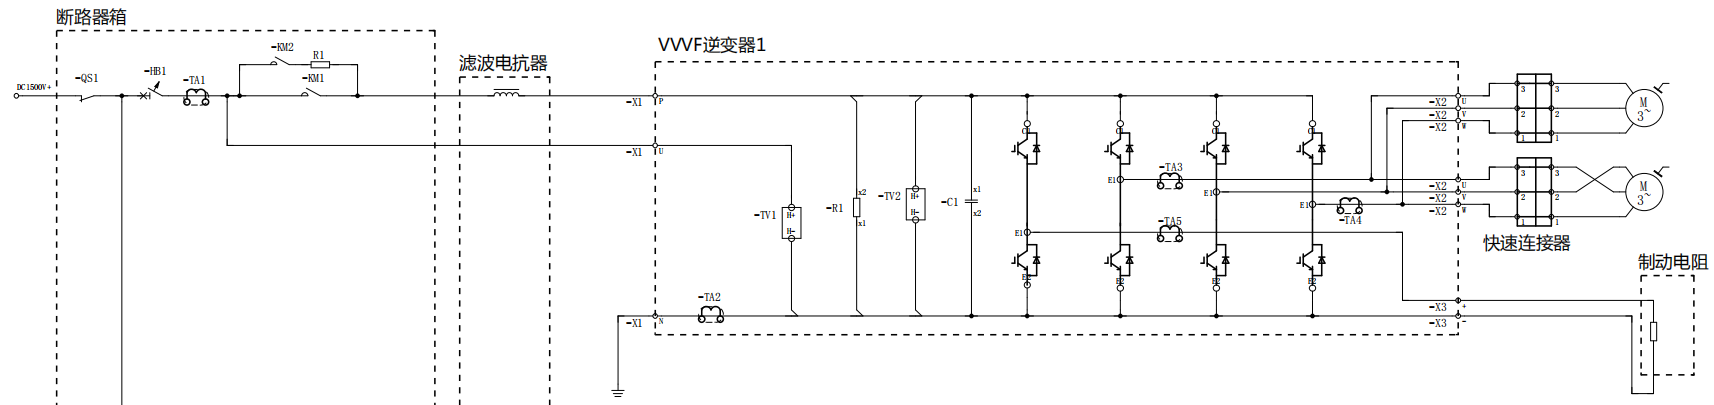
\includegraphics[width=\linewidth]{牵引主电路图.png}
  \caption{牵引主电路图}
  \label{fig:qianyin}
\end{figure}
% !!! 参考数据说明文档
